Målet med brukbarhetstesten er å finne områder der brukeren ikke forstår hvordan
han skal komme seg videre i programflyten, og se at brukeren klarer å finne
den informasjonen han ønsker.

Etter testen ga vi dem et SUS-skjema - System Usability Scale.

Hos Merete scoret vi 4+3+4+4+2 = 17 på 1,3,5,7,9 og 2+3+1+3+4 = 13 på
2,4,6,8,10. Hos Ove scoret vi 3+2+3+3+3 = 14 på 1,3,5,7,9 og 4+4+3+3+4 = 18 på
2,4,6,8,10. Dette ga score (17+13) * 2.5 = 75 for Merete og (14+18) * 2.5 = 80
fra Ove. De to scorene ble altså 75/100 fra Merete og 80/100 fra Ove. Dette gir
et snitt på 77.5/100.

Det er litt interessant og observere at Merete ga høyest poeng på de positivt
ladde spørsmålene, mens Ove ga mest poeng på de negativt ladde spørsmålene.

Mye av den tilbakemeldingen vi fikk etter testen tydet på at det som var mest
uklart var flyten gjennom de forskjellige casene. Det var litt forvirrende når
både case 4 og 5 var avhengige av at case 1 og 2 ble gjort om igjen. Vi burde
nok ha fokusert på å lage mer frittstående caser, slik at vi bedre kunne testet
flyten i programmet, og ikke i casene.

\begin{figure}[obs]
\centering
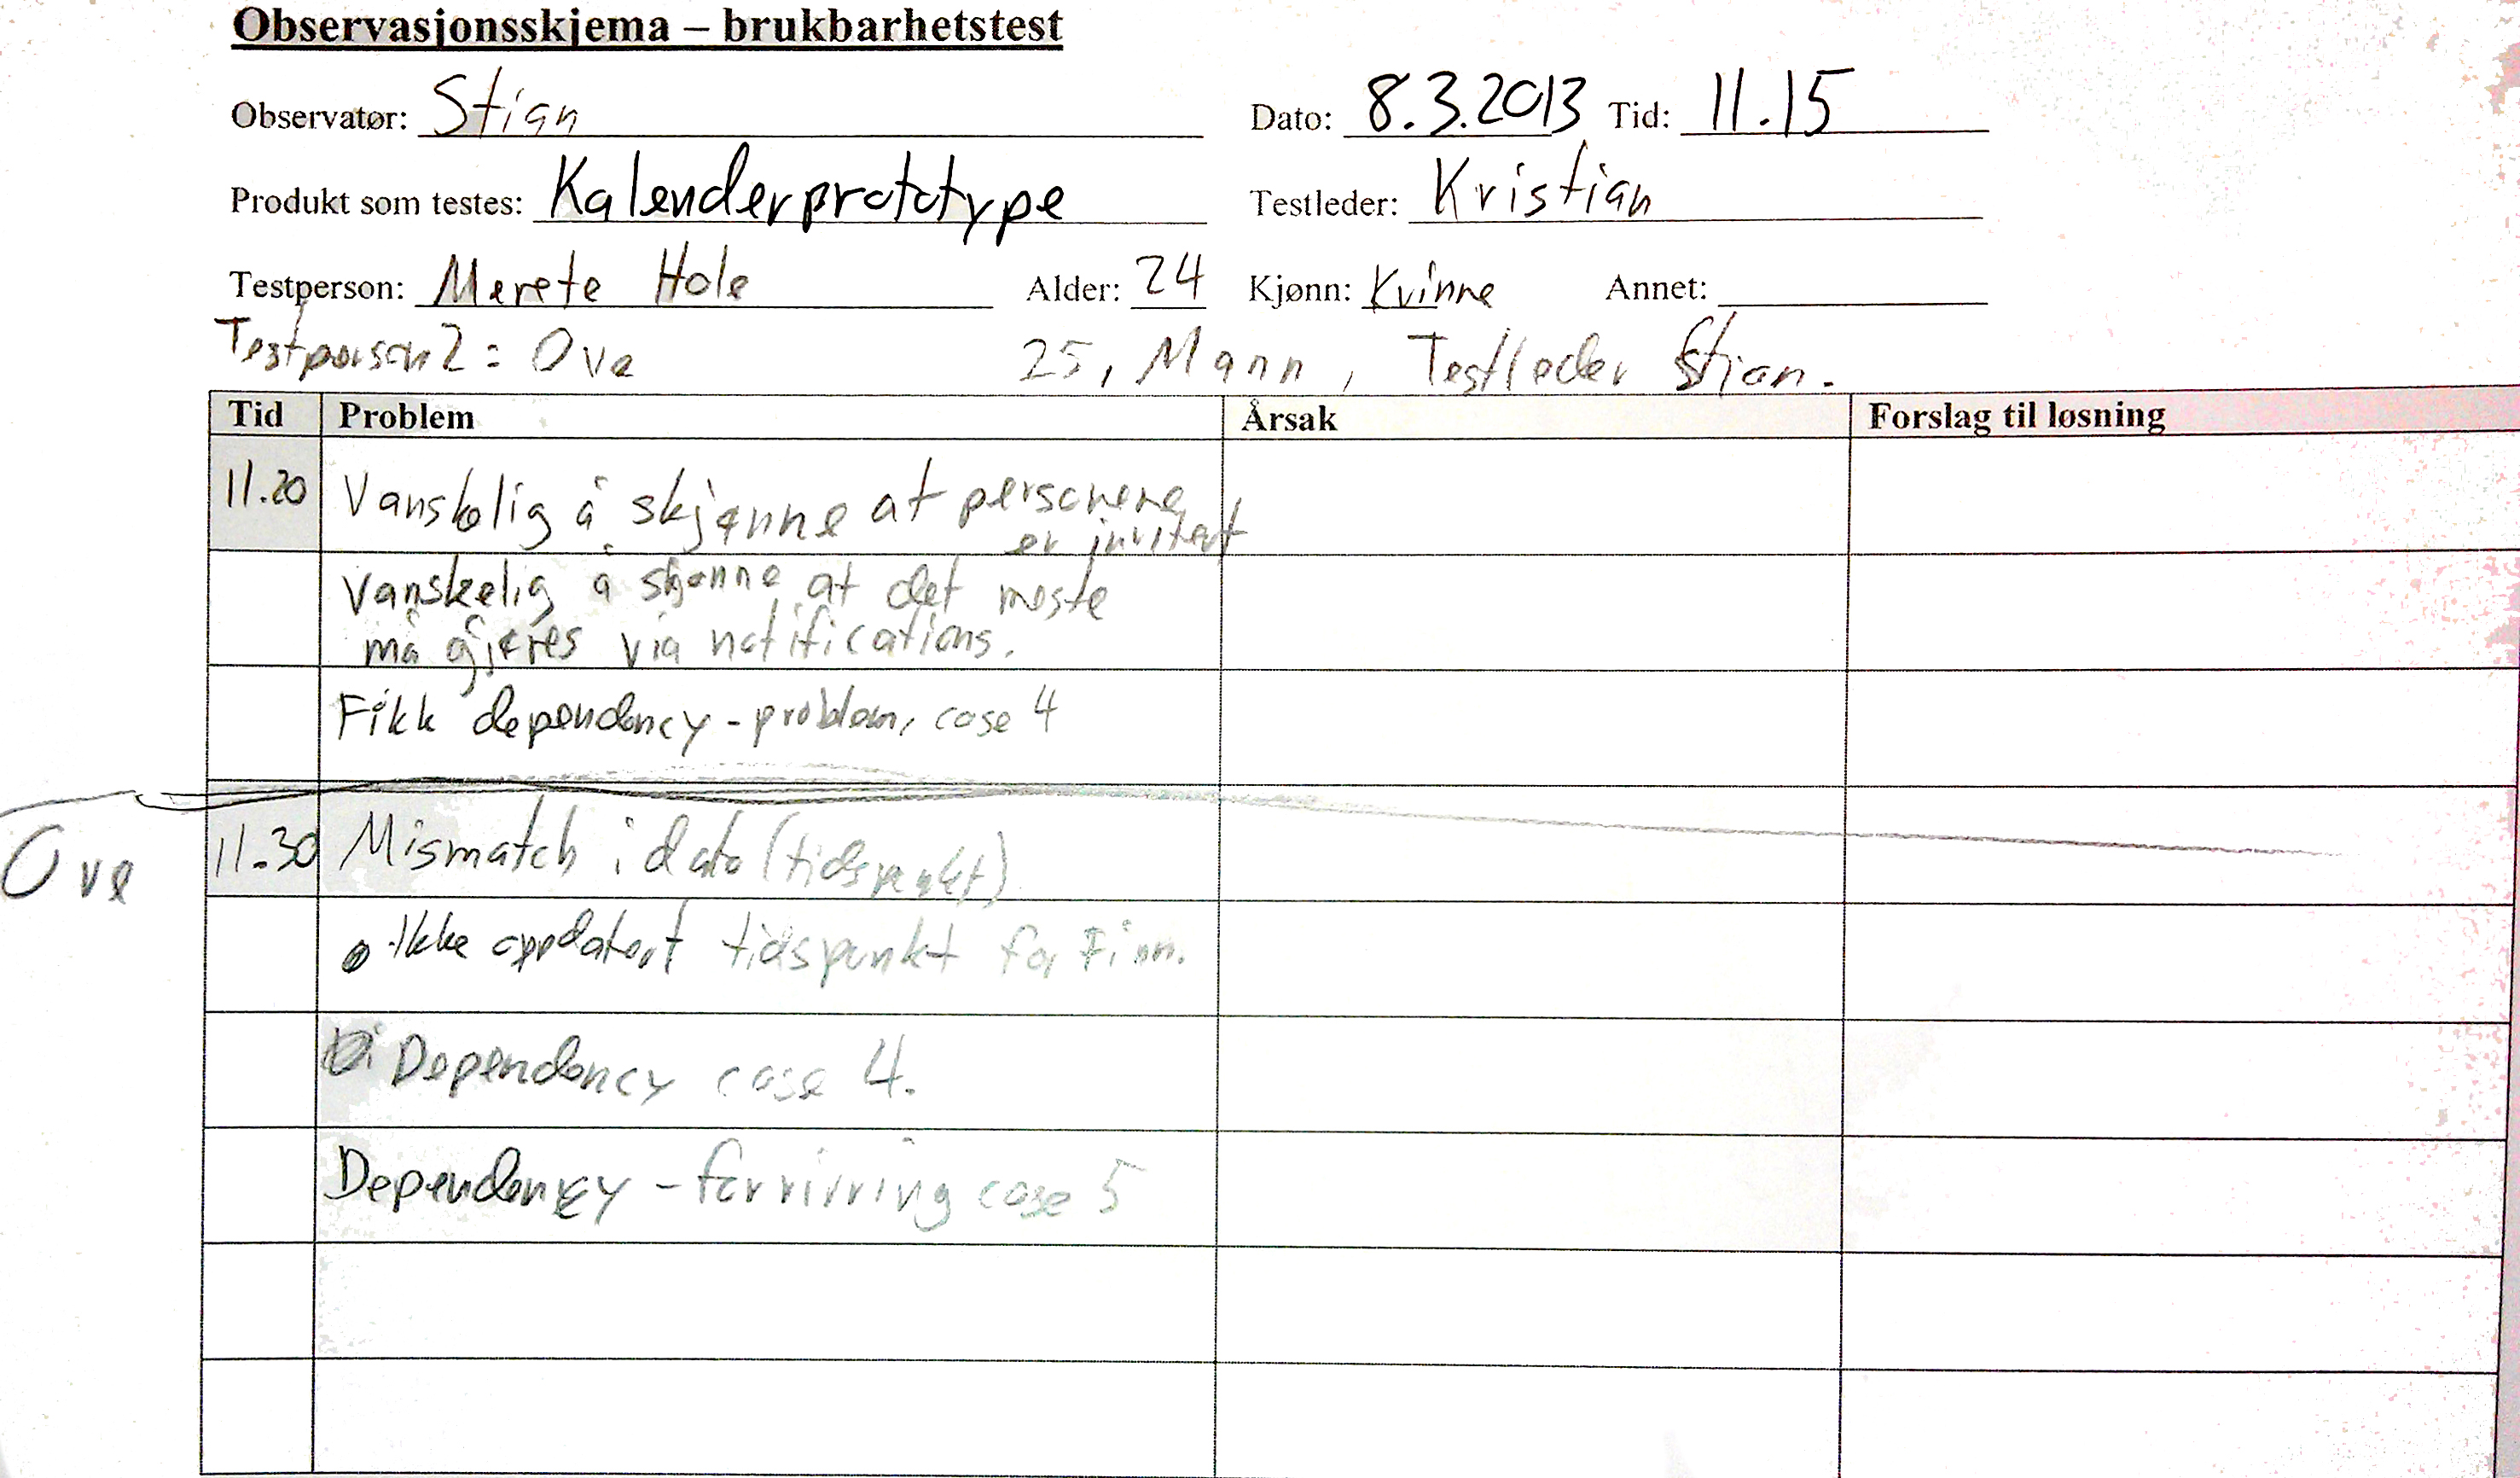
\includegraphics[width=160mm]{images/observasjon.jpg}
\caption{Observasjon}
\label{overflow}
\end{figure}

\begin{figure}[mer]
\centering
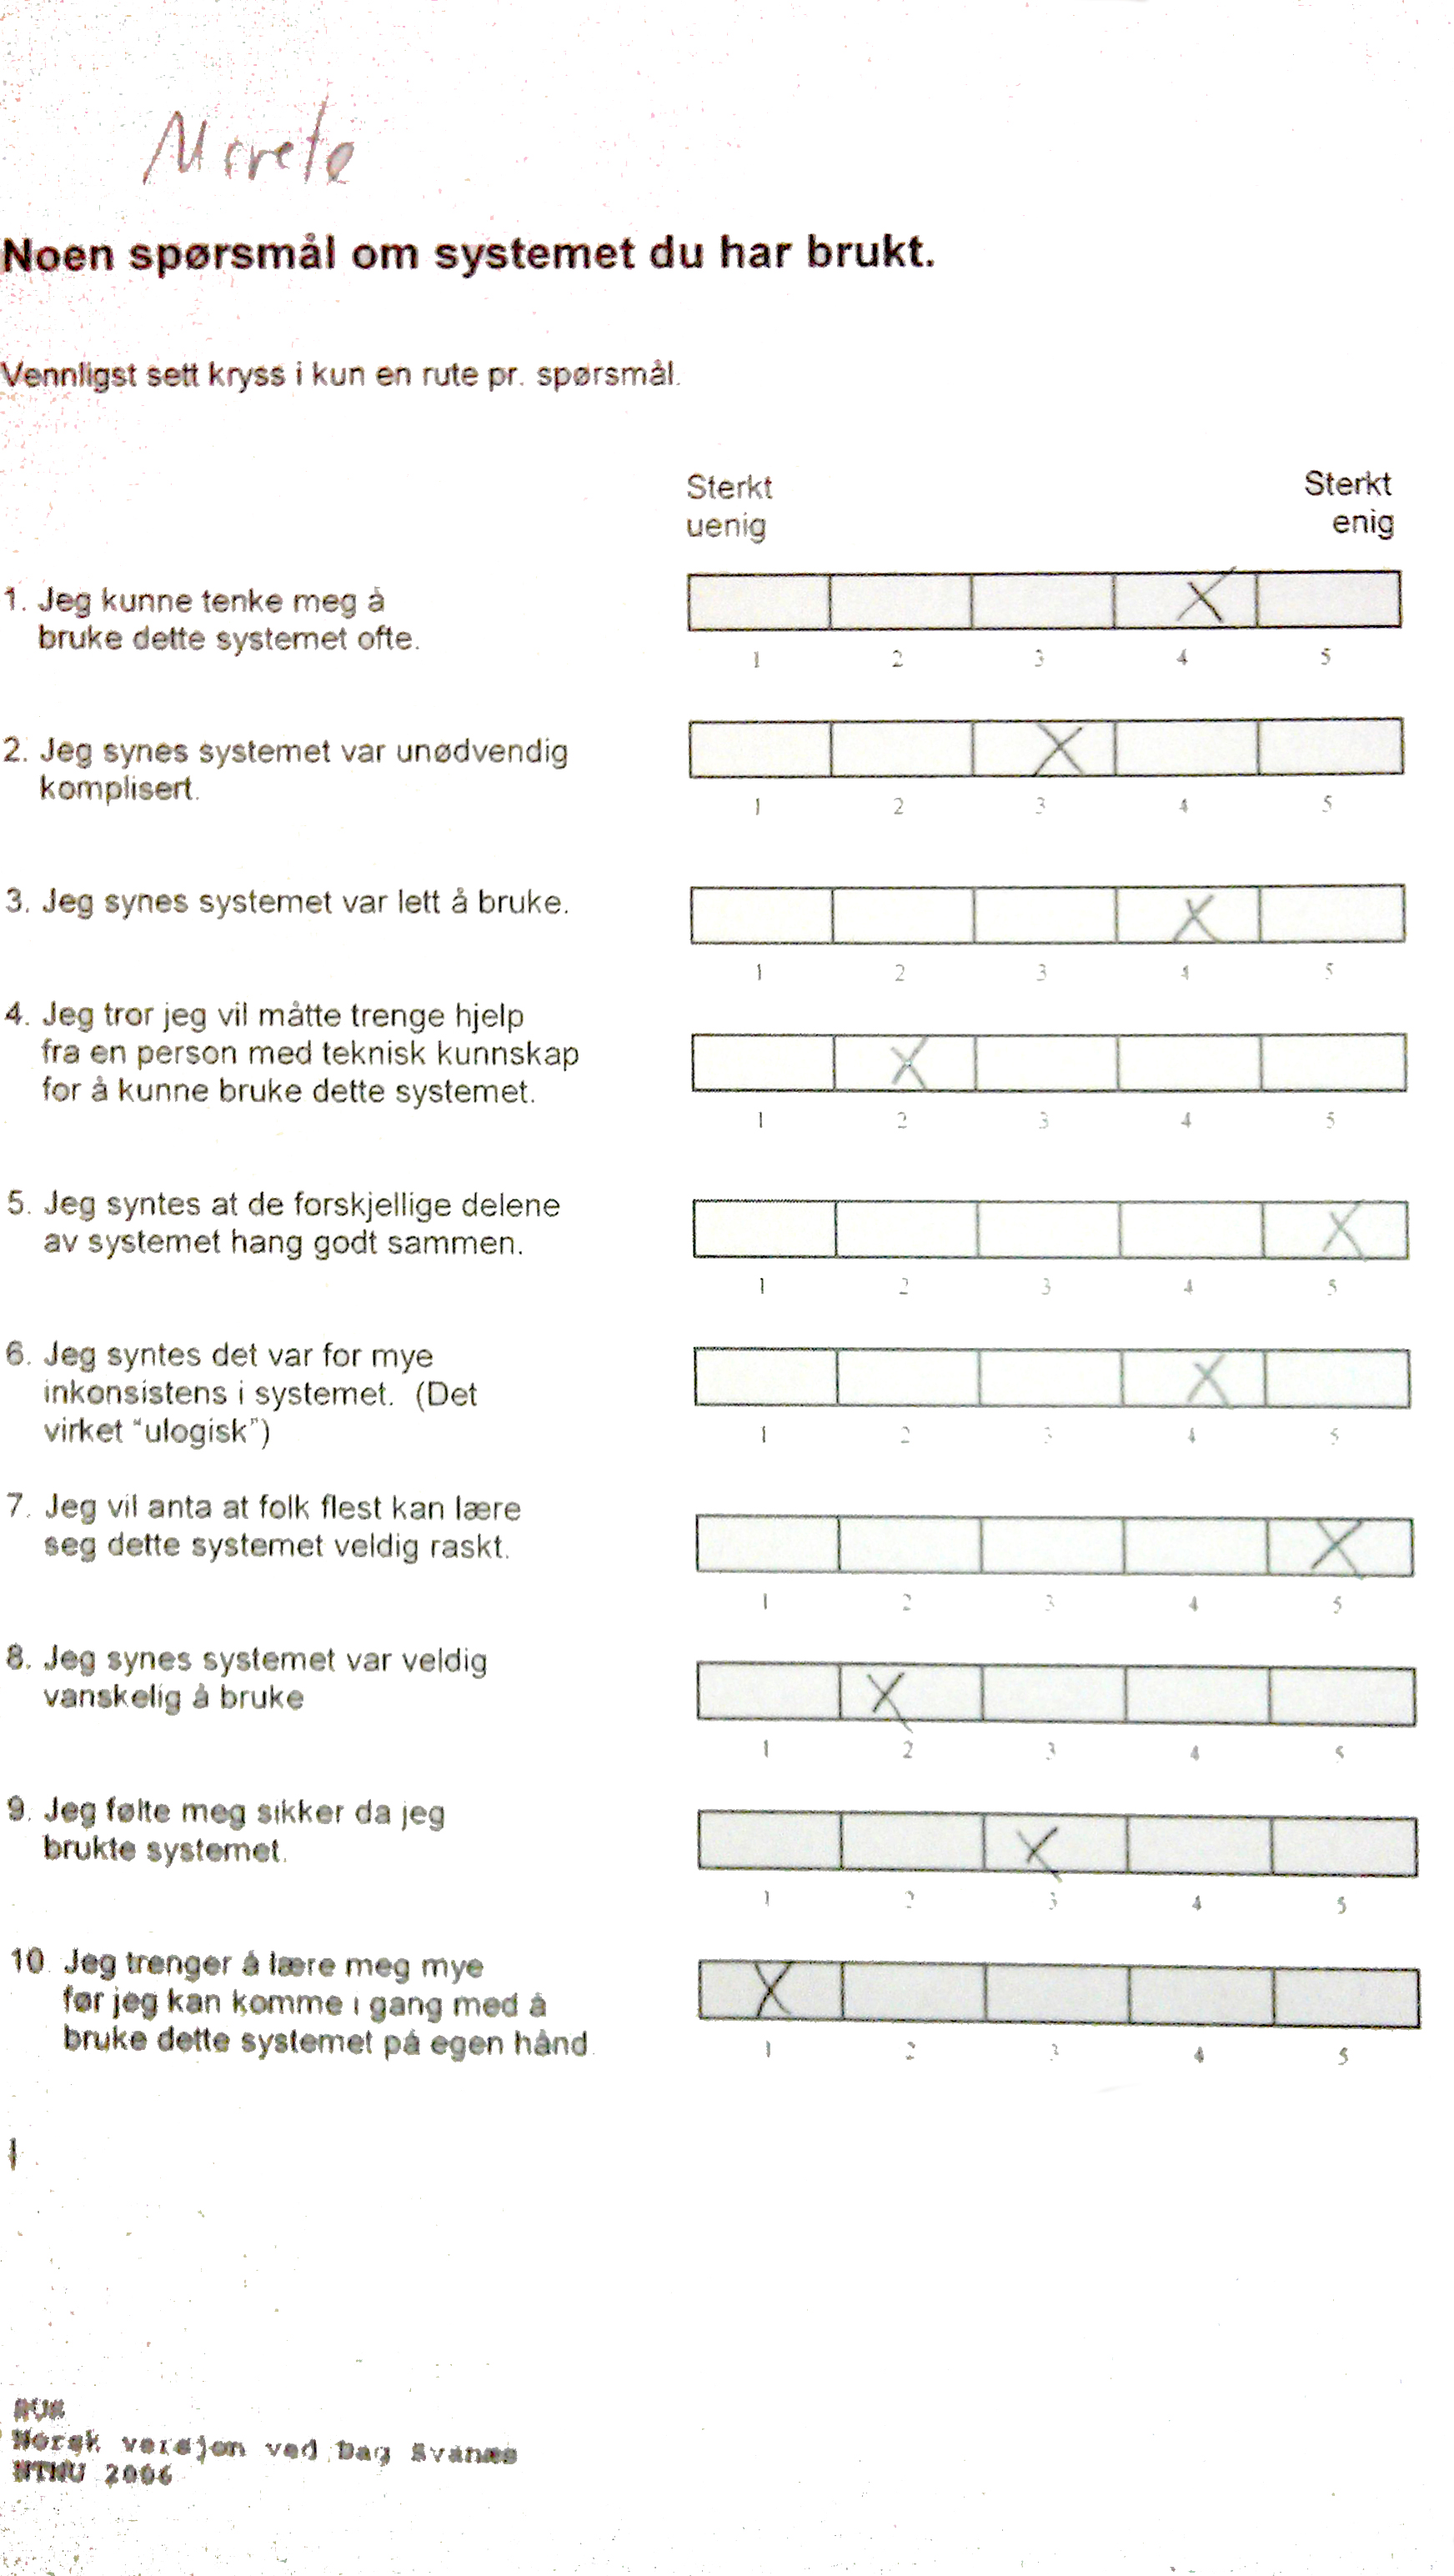
\includegraphics[width=140mm]{images/tilbakemelding_merete.jpg}
\caption{Tilbakemelding fra Merete}
\label{overflow}
\end{figure}

\begin{figure}[ove]
\centering
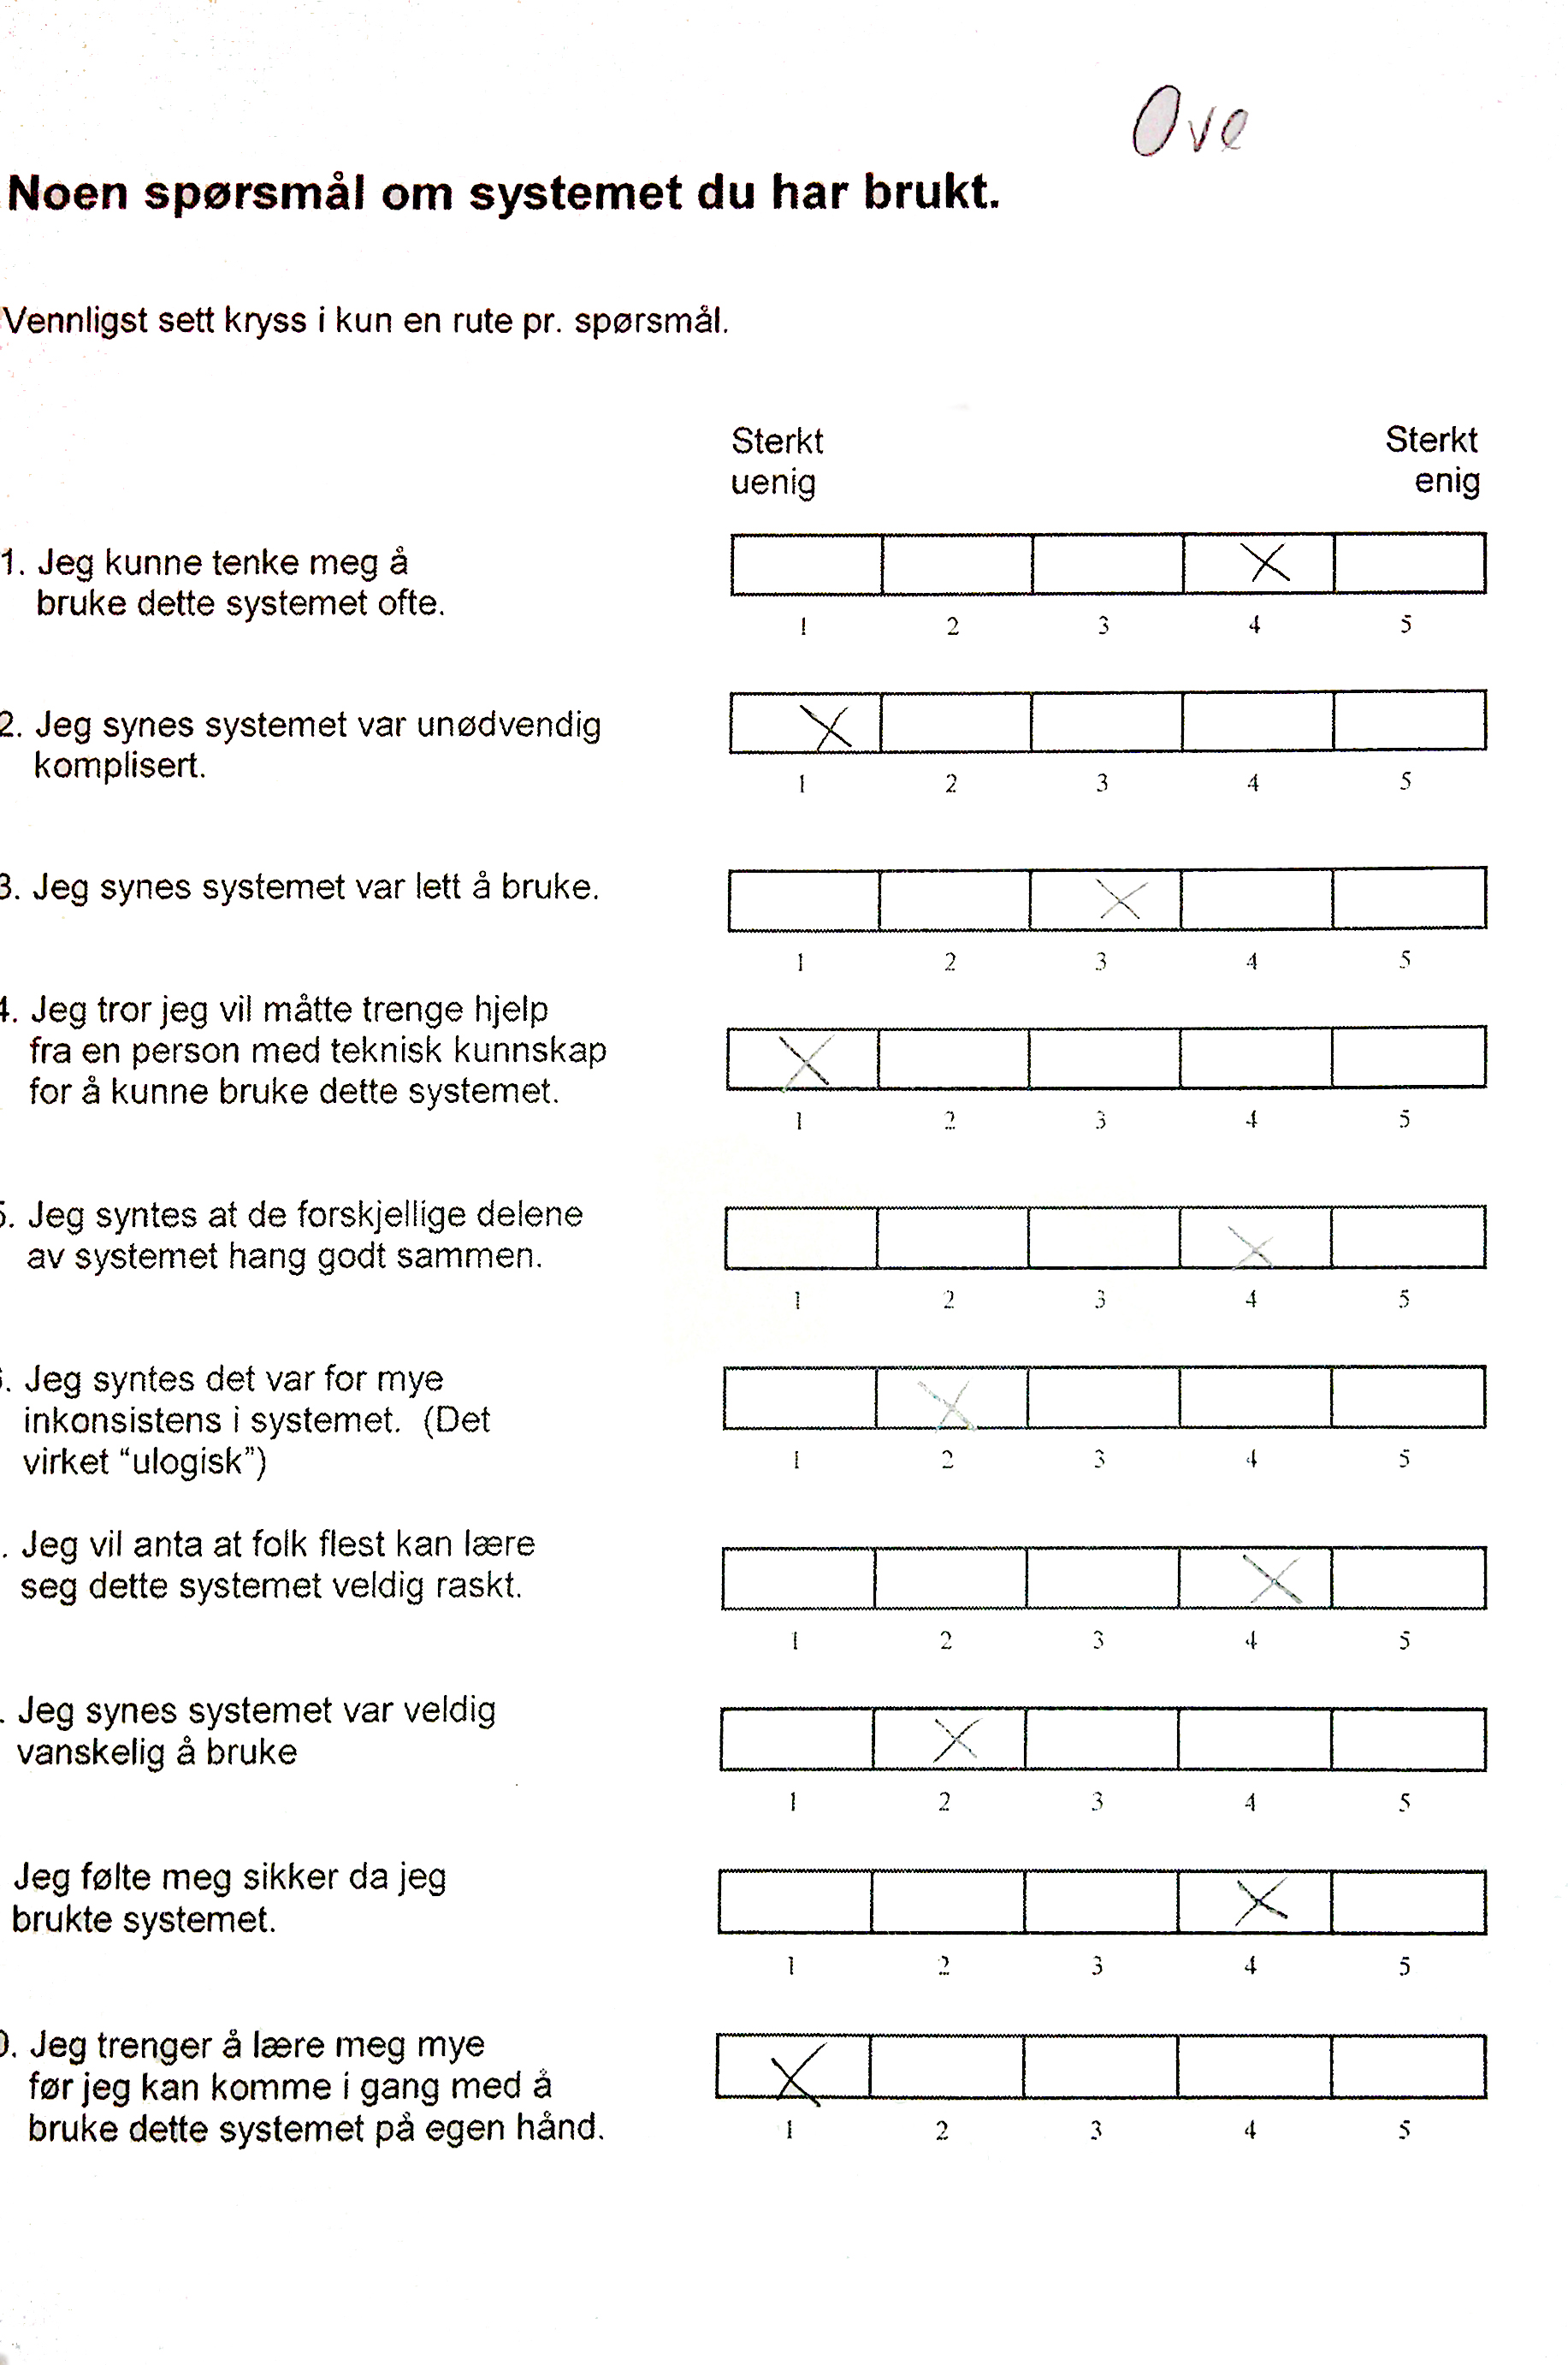
\includegraphics[width=140mm]{images/tilbakemelding_ove.jpg}
\caption{Tibakemelding fra Ove}
\label{overflow}
\end{figure}
